\textbf{ODMR} is a resonance technique by which the electron of a crystal 
defect may be optically excited and its spin state will initialized by the 
spin selection and readout. Among other materials this a method most 
frequently used on diamond has nitrogen vacancy defects (NV). Yet, it is
quite hard to find a comprehensive and clear explanation of the method 
including application details. Here, I will provide detailed information on
our measurement and data processing methods for measuring the ODMR contrast.

\subsection{Data acquisition and initial processing}\label{subsec:dataAcquisition}
Since ODMR method relies on the observation of changes in the PL emission 
spectra of the target material defects, it requires either a spectrometer 
or a photon counting unit like PMT or APD. Our setup utilizes a relatively 
low-profile and low-cost spectrometer from ASEQ Instruments[ref here!!] for
the collection of PL emission. The PL emission from NV diamond is basically  
coupled in to the spectrometer through an optical fiber as it was shown in 
Figure\ref{fig:ConfocalReflectingMicroscopeFull}. This is the raw PL data 
which depending on the setup includes dark background counts produced in the
detector chip, fluorescence background emission produced by the buffer media
where the actual sample resides, and the actual PL emission from the target
material, here NV defects in the diamond. Identification of these emissions 
from different sources and isolation of the PL from NV defects are imperative
for proper quantification ODMR data.

\subsubsection{Spectrometer properties and dark background removal}\label{subsubsec:darkBGMethod}
A spectrometer is a charge coupled device (CCD) which reads out 
photon counts based on their wavelengths. An input light coupled into a
spectrometer either through air or an optical fiber, shines on to a grating 
within the device and diffracted. The diffraction grating separates the 
wavelength components of the light by directing each wavelength into a unique 
output angle. Hence each pixel on the CCD accepts only the photons from a 
particular wavelength range. These photons create electrons on the CCD chip 
units/pixels and the electron counts reported as the photon counts acquired 
per pixel. 

In our experiments we utilized a low-cost portable spectrometer from ASEQ 
Instruments, since these devices are very common and easy to operate. Our
ASEQ spectrometer has a line detector (CCD) TCD1304DG from Toshiba as its 
sensor. This is a 3694 pixel detector and 3654 of them are set to be used 
in a measurement. Currents from CCD are converted to photon counts per pixel 
through a 16 bit analog to digital converter (ADC). Therefore the maximum 
counts per pixel is limited to 65535 (a.k.a. maximum 16 bit unsigned int). 
Analog-to-digital conversion of the CCD's output creates a noise called 
\textbf{read noise} in the measurement. In a typical experiment, at relatively 
integration/exposure times the read noise realized as background counts in
CCD pixels in the absence of input light. This background counts often 
measured and reported by CCD manufacturers by averaging them throughout
the whole chip. Yet every pixel has its unique read noise, so contribute the
background in a different way.  

A common method for cleaning up the actual spectra from background is 
subtracting a snapshot of the these counts which was measured in the absence 
input light. In Figure\ref{fig:BGasIntTimes}, an example of 
background counts we acquired in our system is given as a function of exposure 
times. This is an easy to execute and fast method, and it serves well the 
qualitative analysis of emission/absorption spectra. In case of quantitative 
analysis, a better understanding of the background counts in statistical sense is 
required. To achieve a statistically sound description of background counts at the 
pixel level, one can sample them and attempt to fit a model to count distribution 
of each pixel. Since at the short exposure times the counts expected to be read 
noise dominated, a Gaussian model is usually good enough for fitting the 
distribution. Background count distributions of a random pixel
in our spectrometer given in Figure\ref{fig:BGofRandomPixelasIntTimes}, is a good
example of this behavior. Nevertheless, both by unknown sampling amount
of counts per pixel and by the requirement of manual parameter estimation per
fit, this approach is not practical nor it is straightforward to execute.

\begin{figure}[H]
	\centering
	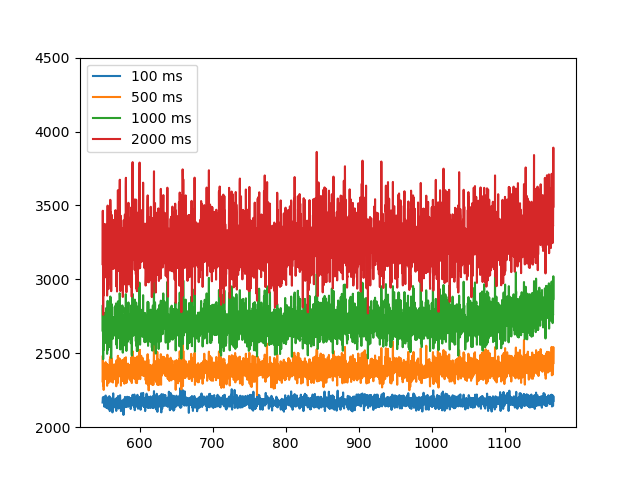
\includegraphics[angle=0,origin=c,width = 1.0\linewidth]{Section_ODMR/Figures/BGCounts_AsFunctionOfIntegrationTime.png}
	\caption{Typical background counts from ASEQ spectrometer as a function of exposure/integration times.}
	\label{fig:BGasIntTimes}
\end{figure}

\begin{figure}[H]
	\centering
	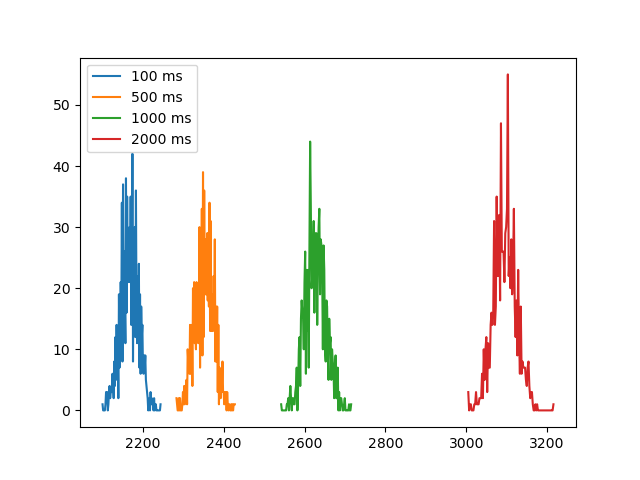
\includegraphics[angle=0,origin=c,width = 1.0\linewidth]{Section_ODMR/Figures/Pixel2550TimeEvolutionOfCounts.png}
	\caption{Count histograms of a random pixel on the CCD as a function of exposure/integration times.}
	\label{fig:BGofRandomPixelasIntTimes}
\end{figure}

To circumvent both problems, we employed a machine learning method called 
expectation-maximization (EM) algorithm to describe background counts of our CCD 
at the pixel level. Under the assumption of Gaussian distributed counts per pixel, 
the algorithm learns the parameters of a Gaussian Mixture Model (GMM) from 
the sampled background data via Bayesian inference. Calculated distributions by GMM
algorithm on the background data of a randomly selected pixel for 5000 shots and the normalized histograms of the actual counts at various exposure times are shown 
in Figures
\ref{fig:BGofRandomPixelasIntTimesFits100ms},\ref{fig:BGofRandomPixelasIntTimesFits500ms}, \ref{fig:BGofRandomPixelasIntTimesFits1000ms}, and \ref{fig:BGofRandomPixelasIntTimesFits2000ms}.

\begin{figure}[H]
	\centering
	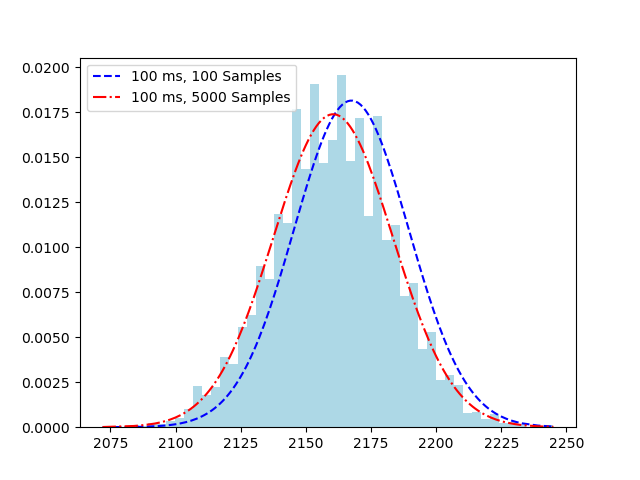
\includegraphics[angle=0,origin=c,width = 0.8\linewidth]{Section_ODMR/Figures/Pixel2550_100msFits.png}
	\caption{Count histograms of a random pixel on the CCD at the 100ms exposure time and GMM fits for low and high
		 sample rates.}
	\label{fig:BGofRandomPixelasIntTimesFits100ms}
\end{figure}

\begin{figure}[H]
	\centering
	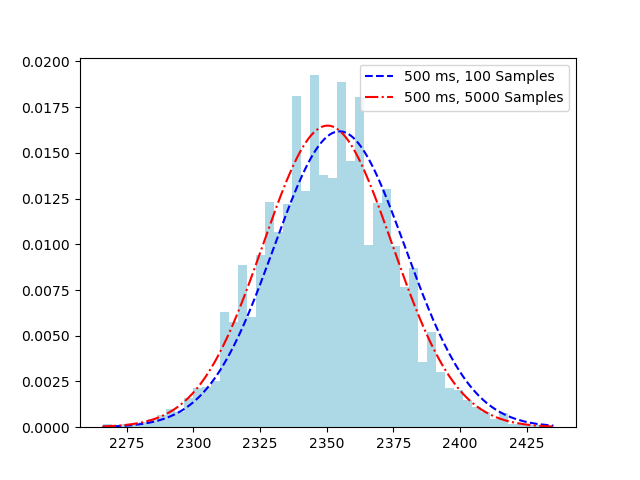
\includegraphics[angle=0,origin=c,width = 0.8\linewidth]{Section_ODMR/Figures/Pixel2550_500msFits.png}
	\caption{Count histograms of a random pixel on the CCD at the 500ms exposure time and GMM fits for low and high
		sample rates.}
	\label{fig:BGofRandomPixelasIntTimesFits500ms}
\end{figure}

\begin{figure}[H]
	\centering
	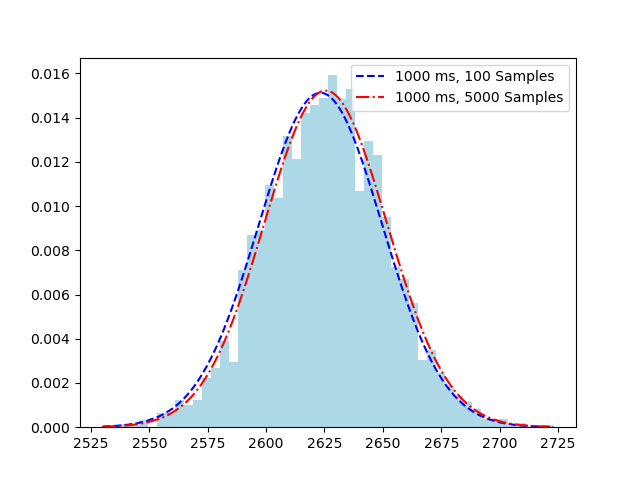
\includegraphics[angle=0,origin=c,width = 0.8\linewidth]{Section_ODMR/Figures/Pixel2550_1000msFits.png}
	\caption{Count histograms of a random pixel on the CCD at the 1000ms exposure time and GMM fits for low and high
		sample rates.}
	\label{fig:BGofRandomPixelasIntTimesFits1000ms}
\end{figure}

\begin{figure}[H]
	\centering
	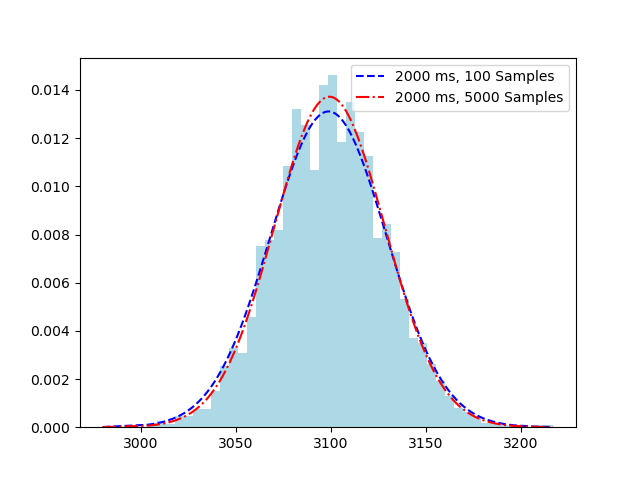
\includegraphics[angle=0,origin=c,width = 0.8\linewidth]{Section_ODMR/Figures/Pixel2550_2000msFits.png}
	\caption{Count histograms of a random pixel on the CCD at the 2000ms exposure time and GMM fits for low and high
		sample rates.}
	\label{fig:BGofRandomPixelasIntTimesFits2000ms}
\end{figure}

As it is shown in the Table\ref{table:test}, estimated GMM parameter 
values change minimally between the sampling size of 100  and 5000 on a
data of 10000 shots. According to the data the worst case estimate occurs
for shorter exposure times not exceeding 7 counts in 2160 for the mean 
value and 1 count in 22 for the standard deviation. This indicates that 
parameters of background counts can be estimated as efficiently by using 
sample sizes of 100 or larger for at least two decades in exposure times
(i.e 100ms to 10000ms).


\begin{table}[h!]
	\centering
	\begin{tabular}{| c | c | c | c | c |} 
		\hline
		 \multirow{2}{*}{Exposure (ms)} & \multicolumn{2} {|c|} {100 Samples} & \multicolumn{2} {|c|} {5000 Samples} \\ 
		\cline{2-5}
		  &  $\mu$ & $\sigma$ & $\mu$ & $\sigma$ \\ 
		\hline
		100 & 2167.5 & 22.0 & 2160.5 & 23.0\\
		\hline
		500 & 2355.0 & 24.7 & 2350.0 & 24.2\\
		\hline
		1000 & 2623.3 & 26.4 & 2625.5 & 26.2\\
		\hline
		2000 & 3098.8 & 29.1 & 3099.3 & 30.4\\
		\hline
	\end{tabular}
	\caption{GMM parameter estimates for large and small sampling sizes as a function
	of exposure times.}
	\label{table:test}
\end{table}

\subsubsection{Fluorescent background removal}\label{subsubsec:fluorecentBGMethod}
Studies on the PL emission of NV defects can be divided into main groups in terms of
the material used. First group is the bulk experiments which utilizes a solid piece of diamond with desired defect densities. The second group nano or micro diamond, 
depending on the experiment, embedded in a solid or liquid media. Although the 
optical measurement systems in these experiments spatially filter most of the 
emission from the environment, some fluorescence couple and contaminate the PL 
spectra in this group of experiments. 

The essential difference between the dark background\ref{subsubsec:darkBGMethod} 
and the fluorescent background is that while the counts from the former follow a 
Gaussian distribution, counts from the latter follows Poisson distibution. In other 
words, the total background in a PL measurement is composed of counts in each pixel 
drawn from statistical distribution which is the convolution of a Gaussian and a 
Poissonian. Since there is no analytical expression for this distribution, we 
facilitate an approximation for cleaning up the PL data. In our method, we first 
define the dark background as explained in Section\ref{subsubsec:darkBGMethod}, 
then we remove the mean counts from the PL data taken in the absence of NV defects 
at the pixel level. The remaining counts at each pixel are supposed to be emitted 
by the environment. We sample these counts to find out the parameters describing 
their distribution at pixel level. In this analysis, we use Poisson Mixtures 
instead of GMM.

\subsection{CW-ODMR measurement and calculation of parameters}
I don't know what to say here!!!
\subsubsection{Cleaning up NV$^{0}$ contribution}
In the context of fluorescence, intersystem crossing (ISC) refers to 
non-emissive transitions pathways that the emitter goes through to return from the 
excited state to its ground state. It is known that the NV centers' excited state 
is a spin triplet, so the excited electron can be in a spin state of $m_{s} = 0$ 
or $\pm$ 1. Among which only the electrons with spins of $m_{s} = \pm 1$ can
undergo ISC. It is also know that ISC is not a spin conserving transition, so 
once an electron experience ISC it does not follow the spin selection rules.
It should also be noted that there are no reported bleaching pathways for NV diamond.
Hence, in contrast to typical fluorophores, ISC creates blinking but the defect 
emission does not stop by a chemical transition. 

Application of microwave field (MW) to NV defects is a well-known method for manipulating the relative populations of electrons in $m_{s} = 0$ and 
$m_{s} = \pm 1$ states. When the applied MW field resonates with the defect 
centers' frequency, it increases the electron population ion $m_{s} = \pm 1$ 
states, so it promotes ISC and reduce the PL intensity. In other words, one can 
monitor PL intensities of NV defects as a function of applied MW field frequencies 
and observe the ratiometric reduction around the resonance frequency. The 
ratiometric change in PL called the \textbf{ODMR contrast}. 

In diamond, individual NV defects can be in either of two charge states, neutral 
NV$^{0}$ and NV$^{-}$. It has been shown that conversion between these states 
occur by light stimulation, and any ensemble of defects have both charge state
populations[REF HERE]. It is also known that the emission spectra of both states 
overlap[REF HERE]. Therefore depending on the excitation wavelength, 
both charge states contribute to the typical PL signal from a diamond sample[REF 
HERE] \ref{fig:rawNVEmission}.

\begin{figure}[H]
	\centering
	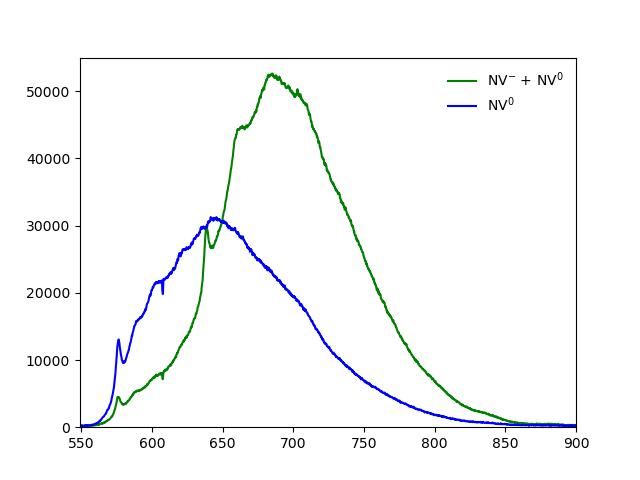
\includegraphics[angle=0,origin=c,width =
	 0.8\linewidth]{Section_ODMR/Figures/rawSpectraNVdefects.png}
	\caption{Emission from ensemble of NV defects by 450nm excitation 
		(blue), and by 532nm excitation (green).}
	\label{fig:rawNVEmission}
\end{figure}

Among NV$^{0}$ and NV$^{-}$, only the latter is reported to be sensitive
to the applied MW field[REF HERE]. This brings the challenge of eliminating
the contribution of NV$^{0}$ defects to the PL data. One method to achieve
this is the excitation of defects by a light source around the ZPL line of
NV$^{-}$ defects which is around 638nm [REF HERE]. As an alternative, 
excitation of NV ensemble by a light source with the wavelength around 450nm
results in a PL of essentially NV$^{0}$ defects. That allows removal of 
NV$^{0}$ contribution from spectra of both types of defects via simple 
scaling \ref{fig:cleanedUpSpectraNVdefects}. Here the scaling can be found by 
the comparison of spectra in the range from 560nm to 595nm [REF HERE].

\begin{figure}[H]
	\centering
	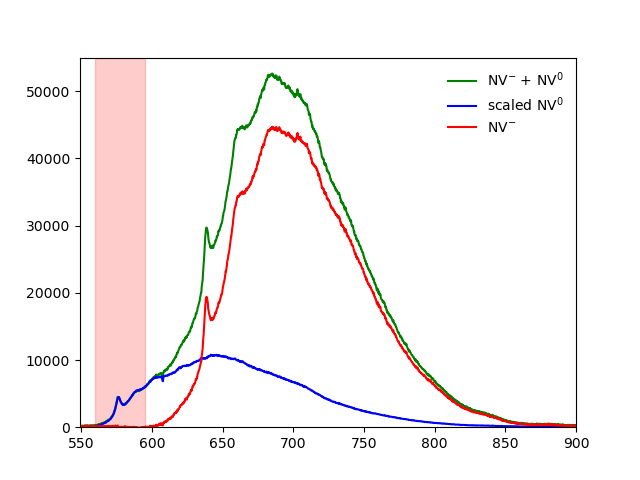
\includegraphics[angle=0,origin=c,width =
	0.8\linewidth]{Section_ODMR/Figures/cleanedUpSpectraNVdefects.png}
	\caption{Emission from ensemble of NV defects by 532nm excitation 
		(green), scaled emission by 450nm excitation (blue), cleaned up
		NV$^{-}$ emission (red). Red shadowed area indicates the region
		of spectra used in the scaling.}
	\label{fig:cleanedUpSpectraNVdefects}
\end{figure}

Since ODMR is the ratiometric change in the PL of NV$^{-}$, it has to take
into consideration of all emission associated with this particular defect.
This translates into the following representation of ODMR based on a PL 
data acquired by a spectrometer;


\begin{equation}
	ODMR = \frac{\sum\limits_{i=\lambda_{min}}^{\lambda_{max}} PL(\lambda_{i})}{max({\sum\limits_{i=\lambda_{min}}^{\lambda_{max}} PL(\lambda_{i})})}
\label{eq:ODMREquation}
\end{equation}

In our knowledge the eq.\ref{eq:ODMREquation} is not given explicitly in 
the literature, but it is mentioned in a handful places [REF HERE!].
The effect of the removal of NV$^{0}$ contribution is shown in
Fig\ref{fig:ODMRBeforeAfterCleanUP}. In the figure, ODMR is calculated 
with and without NV$^{0}$ contribution using $\lambda_{min}=605$nm and 
$\lambda_{max}=885$nm.

\begin{figure}[H]
	\centering
	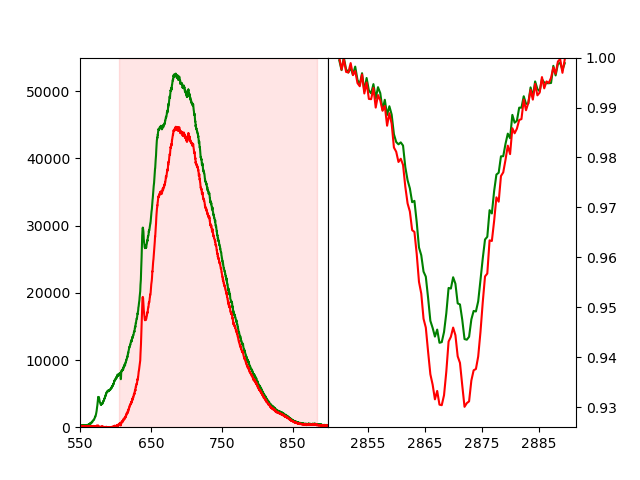
\includegraphics[angle=0,origin=c,width =
	1.0\linewidth]{Section_ODMR/Figures/ODMRAndCleanedUpODMR.png}
	\caption{\textbf{Left} is the PL from ensemble of NV defects by 532nm
		excitation with (green) and without (red) NV$^{0}$ contribution. 
		Shaded area shows the ODMR calculation limits. \textbf{Right} is the 
		calculated ODMR from same color spectra.}
	\label{fig:ODMRBeforeAfterCleanUP}
\end{figure}

\subsubsection{Correction for laser fluctuations and sample heating}
AAAAA

%%\ref{subsec:dataAcquisition}
%Since ODMR method relies on the observation of changes in the PL emission 
%spectra of the target material defects, it requires either a spectrometer 
%or a photon counting unit like PMT or APD. Our setup utilizes a relatively 
%low-profile and low-cost spectrometer from ASEQ Instruments[ref here!!] for
%the collection of PL emission. The PL emission from NV diamond is basically  
%coupled in to the spectrometer through an optical fiber as it was shown in 
%Figure\ref{fig:ConfocalReflectingMicroscopeFull}. This is the raw PL data 
%which depending on the setup includes dark background counts produced in the
%detector chip, fluorescence background emission produced by the buffer media
%where the actual sample resides, and the actual PL emission from the target
%material, here NV defects in the diamond. Identification of these emissions 
%from different sources and isolation of the PL from NV defects are imperative
%for proper quantification ODMR data.

